\documentclass[1p]{elsarticle_modified}
%\bibliographystyle{elsarticle-num}

%\usepackage[colorlinks]{hyperref}
%\usepackage{abbrmath_seonhwa} %\Abb, \Ascr, \Acal ,\Abf, \Afrak
\usepackage{amsfonts}
\usepackage{amssymb}
\usepackage{amsmath}
\usepackage{amsthm}
\usepackage{scalefnt}
\usepackage{amsbsy}
\usepackage{kotex}
\usepackage{caption}
\usepackage{subfig}
\usepackage{color}
\usepackage{graphicx}
\usepackage{xcolor} %% white, black, red, green, blue, cyan, magenta, yellow
\usepackage{float}
\usepackage{setspace}
\usepackage{hyperref}

\usepackage{tikz}
\usetikzlibrary{arrows}

\usepackage{multirow}
\usepackage{array} % fixed length table
\usepackage{hhline}

%%%%%%%%%%%%%%%%%%%%%
\makeatletter
\renewcommand*\env@matrix[1][\arraystretch]{%
	\edef\arraystretch{#1}%
	\hskip -\arraycolsep
	\let\@ifnextchar\new@ifnextchar
	\array{*\c@MaxMatrixCols c}}
\makeatother %https://tex.stackexchange.com/questions/14071/how-can-i-increase-the-line-spacing-in-a-matrix
%%%%%%%%%%%%%%%

\usepackage[normalem]{ulem}

\newcommand{\msout}[1]{\ifmmode\text{\sout{\ensuremath{#1}}}\else\sout{#1}\fi}
%SOURCE: \msout is \stkout macro in https://tex.stackexchange.com/questions/20609/strikeout-in-math-mode

\newcommand{\cancel}[1]{
	\ifmmode
	{\color{red}\msout{#1}}
	\else
	{\color{red}\sout{#1}}
	\fi
}

\newcommand{\add}[1]{
	{\color{blue}\uwave{#1}}
}

\newcommand{\replace}[2]{
	\ifmmode
	{\color{red}\msout{#1}}{\color{blue}\uwave{#2}}
	\else
	{\color{red}\sout{#1}}{\color{blue}\uwave{#2}}
	\fi
}

\newcommand{\Sol}{\mathcal{S}} %segment
\newcommand{\D}{D} %diagram
\newcommand{\A}{\mathcal{A}} %arc


%%%%%%%%%%%%%%%%%%%%%%%%%%%%%5 test

\def\sl{\operatorname{\textup{SL}}(2,\Cbb)}
\def\psl{\operatorname{\textup{PSL}}(2,\Cbb)}
\def\quan{\mkern 1mu \triangleright \mkern 1mu}

\theoremstyle{definition}
\newtheorem{thm}{Theorem}[section]
\newtheorem{prop}[thm]{Proposition}
\newtheorem{lem}[thm]{Lemma}
\newtheorem{ques}[thm]{Question}
\newtheorem{cor}[thm]{Corollary}
\newtheorem{defn}[thm]{Definition}
\newtheorem{exam}[thm]{Example}
\newtheorem{rmk}[thm]{Remark}
\newtheorem{alg}[thm]{Algorithm}

\newcommand{\I}{\sqrt{-1}}
\begin{document}

%\begin{frontmatter}
%
%\title{Boundary parabolic representations of knots up to 8 crossings}
%
%%% Group authors per affiliation:
%\author{Yunhi Cho} 
%\address{Department of Mathematics, University of Seoul, Seoul, Korea}
%\ead{yhcho@uos.ac.kr}
%
%
%\author{Seonhwa Kim} %\fnref{s_kim}}
%\address{Center for Geometry and Physics, Institute for Basic Science, Pohang, 37673, Korea}
%\ead{ryeona17@ibs.re.kr}
%
%\author{Hyuk Kim}
%\address{Department of Mathematical Sciences, Seoul National University, Seoul 08826, Korea}
%\ead{hyukkim@snu.ac.kr}
%
%\author{Seokbeom Yoon}
%\address{Department of Mathematical Sciences, Seoul National University, Seoul, 08826,  Korea}
%\ead{sbyoon15@snu.ac.kr}
%
%\begin{abstract}
%We find all boundary parabolic representation of knots up to 8 crossings.
%
%\end{abstract}
%\begin{keyword}
%    \MSC[2010] 57M25 
%\end{keyword}
%
%\end{frontmatter}

%\linenumbers
%\tableofcontents
%
\newcommand\colored[1]{\textcolor{white}{\rule[-0.35ex]{0.8em}{1.4ex}}\kern-0.8em\color{red} #1}%
%\newcommand\colored[1]{\textcolor{white}{ #1}\kern-2.17ex	\textcolor{white}{ #1}\kern-1.81ex	\textcolor{white}{ #1}\kern-2.15ex\color{red}#1	}

{\Large $\underline{10_{92}~(K10a_{46})}$}

\setlength{\tabcolsep}{10pt}
\renewcommand{\arraystretch}{1.6}
\vspace{1cm}\begin{tabular}{m{100pt}>{\centering\arraybackslash}m{274pt}}
\multirow{5}{120pt}{
	\centering
	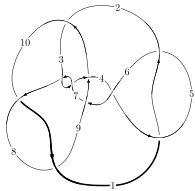
\includegraphics[width=112pt]{../../../GIT/diagram.site/Diagrams/png/176_10_92.png}\\
\ \ \ A knot diagram\footnotemark}&
\allowdisplaybreaks
\textbf{Linearized knot diagam} \\
\cline{2-2}
 &
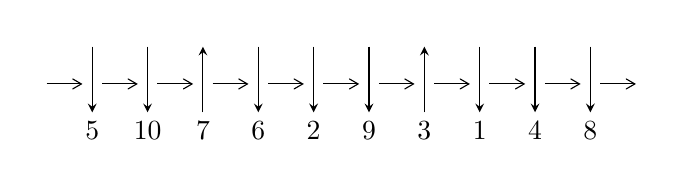
\begin{tikzpicture}[x=20pt, y=17pt]
	% nodes
	\node (C0) at (0, 0) {};
	\node (C1) at (1, 0) {};
	\node (C1U) at (1, +1) {};
	\node (C1D) at (1, -1) {5};

	\node (C2) at (2, 0) {};
	\node (C2U) at (2, +1) {};
	\node (C2D) at (2, -1) {10};

	\node (C3) at (3, 0) {};
	\node (C3U) at (3, +1) {};
	\node (C3D) at (3, -1) {7};

	\node (C4) at (4, 0) {};
	\node (C4U) at (4, +1) {};
	\node (C4D) at (4, -1) {6};

	\node (C5) at (5, 0) {};
	\node (C5U) at (5, +1) {};
	\node (C5D) at (5, -1) {2};

	\node (C6) at (6, 0) {};
	\node (C6U) at (6, +1) {};
	\node (C6D) at (6, -1) {9};

	\node (C7) at (7, 0) {};
	\node (C7U) at (7, +1) {};
	\node (C7D) at (7, -1) {3};

	\node (C8) at (8, 0) {};
	\node (C8U) at (8, +1) {};
	\node (C8D) at (8, -1) {1};

	\node (C9) at (9, 0) {};
	\node (C9U) at (9, +1) {};
	\node (C9D) at (9, -1) {4};

	\node (C10) at (10, 0) {};
	\node (C10U) at (10, +1) {};
	\node (C10D) at (10, -1) {8};
	\node (C11) at (11, 0) {};

	% arrows
	\draw[->,>={angle 60}]
	(C0) edge (C1) (C1) edge (C2) (C2) edge (C3) (C3) edge (C4) (C4) edge (C5) (C5) edge (C6) (C6) edge (C7) (C7) edge (C8) (C8) edge (C9) (C9) edge (C10) (C10) edge (C11) ;	\draw[->,>=stealth]
	(C1U) edge (C1D) (C2U) edge (C2D) (C3D) edge (C3U) (C4U) edge (C4D) (C5U) edge (C5D) (C6U) edge (C6D) (C7D) edge (C7U) (C8U) edge (C8D) (C9U) edge (C9D) (C10U) edge (C10D) ;
	\end{tikzpicture} \\
\hhline{~~} \\& 
\textbf{Solving Sequence} \\ \cline{2-2} 
 &
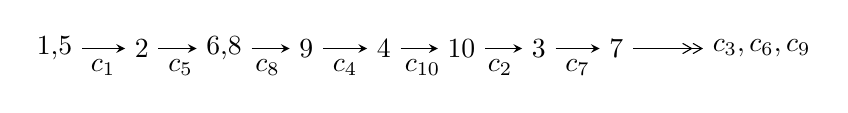
\begin{tikzpicture}[x=28pt, y=7pt]
	% node
	\node (A0) at (-1/8, 0) {1,5};
	\node (A1) at (1, 0) {2};
	\node (A2) at (33/16, 0) {6,8};
	\node (A3) at (25/8, 0) {9};
	\node (A4) at (33/8, 0) {4};
	\node (A5) at (41/8, 0) {10};
	\node (A6) at (49/8, 0) {3};
	\node (A7) at (57/8, 0) {7};
	\node (C1) at (1/2, -1) {$c_{1}$};
	\node (C2) at (3/2, -1) {$c_{5}$};
	\node (C3) at (21/8, -1) {$c_{8}$};
	\node (C4) at (29/8, -1) {$c_{4}$};
	\node (C5) at (37/8, -1) {$c_{10}$};
	\node (C6) at (45/8, -1) {$c_{2}$};
	\node (C7) at (53/8, -1) {$c_{7}$};
	\node (A8) at (9, 0) {$c_{3},c_{6},c_{9}$};

	% edge
	\draw[->,>=stealth]	
	(A0) edge (A1) (A1) edge (A2) (A2) edge (A3) (A3) edge (A4) (A4) edge (A5) (A5) edge (A6) (A6) edge (A7) ;
	\draw[->>,>={angle 60}]	
	(A7) edge (A8);
\end{tikzpicture} \\ 

\end{tabular} \\

\footnotetext{
The image of knot diagram is generated by the software ``\textbf{Draw programme}" developed by Andrew Bartholomew(\url{http://www.layer8.co.uk/maths/draw/index.htm\#Running-draw}), where we modified some parts for our purpose(\url{https://github.com/CATsTAILs/LinksPainter}).
}\phantom \\ \newline 
\centering \textbf{Ideals for irreducible components\footnotemark of $X_{\text{par}}$} 
 
\begin{align*}
I^u_{1}&=\langle 
6.14745\times10^{22} u^{43}+1.68640\times10^{23} u^{42}+\cdots+4.10626\times10^{23} b+5.65855\times10^{23},\\
\phantom{I^u_{1}}&\phantom{= \langle  }-1.07830\times10^{23} u^{43}-7.28908\times10^{23} u^{42}+\cdots+4.10626\times10^{23} a-8.55134\times10^{23},\;u^{44}+3 u^{43}+\cdots+4 u+1\rangle \\
\\
\end{align*}
\raggedright * 1 irreducible components of $\dim_{\mathbb{C}}=0$, with total 44 representations.\\
\footnotetext{All coefficients of polynomials are rational numbers. But the coefficients are sometimes approximated in decimal forms when there is not enough margin.}
\newpage
\renewcommand{\arraystretch}{1}
\centering \section*{I. $I^u_{1}= \langle 6.15\times10^{22} u^{43}+1.69\times10^{23} u^{42}+\cdots+4.11\times10^{23} b+5.66\times10^{23},\;-1.08\times10^{23} u^{43}-7.29\times10^{23} u^{42}+\cdots+4.11\times10^{23} a-8.55\times10^{23},\;u^{44}+3 u^{43}+\cdots+4 u+1 \rangle$}
\flushleft \textbf{(i) Arc colorings}\\
\begin{tabular}{m{7pt} m{180pt} m{7pt} m{180pt} }
\flushright $a_{1}=$&$\begin{pmatrix}1\\0\end{pmatrix}$ \\
\flushright $a_{5}=$&$\begin{pmatrix}0\\u\end{pmatrix}$ \\
\flushright $a_{2}=$&$\begin{pmatrix}1\\u^2\end{pmatrix}$ \\
\flushright $a_{6}=$&$\begin{pmatrix}- u\\- u^3+u\end{pmatrix}$ \\
\flushright $a_{8}=$&$\begin{pmatrix}0.262600 u^{43}+1.77511 u^{42}+\cdots+2.77682 u+2.08251\\-0.149709 u^{43}-0.410691 u^{42}+\cdots-1.54325 u-1.37803\end{pmatrix}$ \\
\flushright $a_{9}=$&$\begin{pmatrix}0.412309 u^{43}+2.18580 u^{42}+\cdots+4.32007 u+3.46054\\-0.149709 u^{43}-0.410691 u^{42}+\cdots-1.54325 u-1.37803\end{pmatrix}$ \\
\flushright $a_{4}=$&$\begin{pmatrix}u^3\\u^5- u^3+u\end{pmatrix}$ \\
\flushright $a_{10}=$&$\begin{pmatrix}0.313341 u^{43}+1.90111 u^{42}+\cdots+3.81262 u+3.26735\\-0.334825 u^{43}-0.772241 u^{42}+\cdots-1.55972 u-1.27556\end{pmatrix}$ \\
\flushright $a_{3}=$&$\begin{pmatrix}1.07273 u^{43}+1.65129 u^{42}+\cdots+0.120109 u-0.207377\\-0.415470 u^{43}-0.355187 u^{42}+\cdots-2.46813 u+0.118486\end{pmatrix}$ \\
\flushright $a_{7}=$&$\begin{pmatrix}0.942379 u^{43}+5.64956 u^{42}+\cdots-4.55203 u+0.322394\\-0.801791 u^{43}-2.31053 u^{42}+\cdots-2.19230 u-1.54713\end{pmatrix}$\\&\end{tabular}
\flushleft \textbf{(ii) Obstruction class $= -1$}\\~\\
\flushleft \textbf{(iii) Cusp Shapes $= -\frac{299808041105979204994396}{136875388103549877144643} u^{43}-\frac{848702959623216598779576}{136875388103549877144643} u^{42}+\cdots-\frac{27052211834725271707812}{19553626871935696734949} u-\frac{1351235298619022041529338}{136875388103549877144643}$}\\~\\
\newpage\renewcommand{\arraystretch}{1}
\flushleft \textbf{(iv) u-Polynomials at the component}\newline \\
\begin{tabular}{m{50pt}|m{274pt}}
Crossings & \hspace{64pt}u-Polynomials at each crossing \\
\hline $$\begin{aligned}c_{1},c_{5}\end{aligned}$$&$\begin{aligned}
&u^{44}+3 u^{43}+\cdots+4 u+1
\end{aligned}$\\
\hline $$\begin{aligned}c_{2}\end{aligned}$$&$\begin{aligned}
&u^{44}+11 u^{43}+\cdots+2050 u-319
\end{aligned}$\\
\hline $$\begin{aligned}c_{3},c_{7}\end{aligned}$$&$\begin{aligned}
&u^{44}+3 u^{43}+\cdots+4 u+1
\end{aligned}$\\
\hline $$\begin{aligned}c_{4}\end{aligned}$$&$\begin{aligned}
&u^{44}+19 u^{43}+\cdots+10 u+1
\end{aligned}$\\
\hline $$\begin{aligned}c_{6}\end{aligned}$$&$\begin{aligned}
&u^{44}+u^{43}+\cdots-28 u+7
\end{aligned}$\\
\hline $$\begin{aligned}c_{8},c_{10}\end{aligned}$$&$\begin{aligned}
&u^{44}- u^{43}+\cdots-16 u-1
\end{aligned}$\\
\hline $$\begin{aligned}c_{9}\end{aligned}$$&$\begin{aligned}
&u^{44}+u^{43}+\cdots+10 u-1
\end{aligned}$\\
\hline
\end{tabular}\\~\\
\newpage\renewcommand{\arraystretch}{1}
\flushleft \textbf{(v) Riley Polynomials at the component}\newline \\
\begin{tabular}{m{50pt}|m{274pt}}
Crossings & \hspace{64pt}Riley Polynomials at each crossing \\
\hline $$\begin{aligned}c_{1},c_{5}\end{aligned}$$&$\begin{aligned}
&y^{44}-19 y^{43}+\cdots-10 y+1
\end{aligned}$\\
\hline $$\begin{aligned}c_{2}\end{aligned}$$&$\begin{aligned}
&y^{44}-107 y^{43}+\cdots-1901234 y+101761
\end{aligned}$\\
\hline $$\begin{aligned}c_{3},c_{7}\end{aligned}$$&$\begin{aligned}
&y^{44}+33 y^{43}+\cdots-10 y+1
\end{aligned}$\\
\hline $$\begin{aligned}c_{4}\end{aligned}$$&$\begin{aligned}
&y^{44}+13 y^{43}+\cdots-10 y+1
\end{aligned}$\\
\hline $$\begin{aligned}c_{6}\end{aligned}$$&$\begin{aligned}
&y^{44}+77 y^{43}+\cdots-1078 y+49
\end{aligned}$\\
\hline $$\begin{aligned}c_{8},c_{10}\end{aligned}$$&$\begin{aligned}
&y^{44}-31 y^{43}+\cdots-122 y+1
\end{aligned}$\\
\hline $$\begin{aligned}c_{9}\end{aligned}$$&$\begin{aligned}
&y^{44}-3 y^{43}+\cdots-50 y+1
\end{aligned}$\\
\hline
\end{tabular}\\~\\
\newpage\flushleft \textbf{(vi) Complex Volumes and Cusp Shapes}
$$\begin{array}{c|c|c}  
\text{Solutions to }I^u_{1}& \I (\text{vol} + \sqrt{-1}CS) & \text{Cusp shape}\\
 \hline 
\begin{aligned}
u &= \phantom{-}0.363757 + 0.931801 I \\
a &= \phantom{-}0.574314 + 0.152690 I \\
b &= \phantom{-}1.051760 - 0.377630 I\end{aligned}
 & \phantom{-}0.93507 + 3.55591 I & -4.27504 - 5.80144 I \\ \hline\begin{aligned}
u &= \phantom{-}0.363757 - 0.931801 I \\
a &= \phantom{-}0.574314 - 0.152690 I \\
b &= \phantom{-}1.051760 + 0.377630 I\end{aligned}
 & \phantom{-}0.93507 - 3.55591 I & -4.27504 + 5.80144 I \\ \hline\begin{aligned}
u &= \phantom{-}0.918123 + 0.411939 I \\
a &= -2.57013 + 0.48465 I \\
b &= -1.186550 + 0.092828 I\end{aligned}
 & -2.84407 - 1.62243 I & -4.14582 + 4.55154 I \\ \hline\begin{aligned}
u &= \phantom{-}0.918123 - 0.411939 I \\
a &= -2.57013 - 0.48465 I \\
b &= -1.186550 - 0.092828 I\end{aligned}
 & -2.84407 + 1.62243 I & -4.14582 - 4.55154 I \\ \hline\begin{aligned}
u &= -0.441228 + 0.915243 I \\
a &= \phantom{-}0.398119 - 0.217535 I \\
b &= \phantom{-}1.34117 + 0.51864 I\end{aligned}
 & -4.18962 - 9.08760 I & -8.08222 + 5.03295 I \\ \hline\begin{aligned}
u &= -0.441228 - 0.915243 I \\
a &= \phantom{-}0.398119 + 0.217535 I \\
b &= \phantom{-}1.34117 - 0.51864 I\end{aligned}
 & -4.18962 + 9.08760 I & -8.08222 - 5.03295 I \\ \hline\begin{aligned}
u &= \phantom{-}0.822616 + 0.487506 I \\
a &= \phantom{-}2.41823 - 5.79626 I \\
b &= -0.962457 - 0.015339 I\end{aligned}
 & -3.21593 - 2.04361 I & -52.4053 - 14.7990 I \\ \hline\begin{aligned}
u &= \phantom{-}0.822616 - 0.487506 I \\
a &= \phantom{-}2.41823 + 5.79626 I \\
b &= -0.962457 + 0.015339 I\end{aligned}
 & -3.21593 + 2.04361 I & -52.4053 + 14.7990 I \\ \hline\begin{aligned}
u &= \phantom{-}0.614573 + 0.715877 I \\
a &= \phantom{-}0.648178 - 0.462248 I \\
b &= \phantom{-}0.352533 + 0.684267 I\end{aligned}
 & \phantom{-}3.04550 - 0.49268 I & -0.12697 + 2.02865 I \\ \hline\begin{aligned}
u &= \phantom{-}0.614573 - 0.715877 I \\
a &= \phantom{-}0.648178 + 0.462248 I \\
b &= \phantom{-}0.352533 - 0.684267 I\end{aligned}
 & \phantom{-}3.04550 + 0.49268 I & -0.12697 - 2.02865 I\\
 \hline 
 \end{array}$$\newpage$$\begin{array}{c|c|c}  
\text{Solutions to }I^u_{1}& \I (\text{vol} + \sqrt{-1}CS) & \text{Cusp shape}\\
 \hline 
\begin{aligned}
u &= \phantom{-}0.925118 + 0.134958 I \\
a &= \phantom{-}0.268380 + 0.914669 I \\
b &= -0.612800 + 0.910777 I\end{aligned}
 & -4.44447 + 2.34717 I & -13.36025 - 3.31347 I \\ \hline\begin{aligned}
u &= \phantom{-}0.925118 - 0.134958 I \\
a &= \phantom{-}0.268380 - 0.914669 I \\
b &= -0.612800 - 0.910777 I\end{aligned}
 & -4.44447 - 2.34717 I & -13.36025 + 3.31347 I \\ \hline\begin{aligned}
u &= -1.006040 + 0.358502 I \\
a &= -1.64888 - 1.39073 I \\
b &= -1.72272 - 0.34047 I\end{aligned}
 & -7.32531 + 1.01598 I & -16.3773 - 1.5947 I \\ \hline\begin{aligned}
u &= -1.006040 - 0.358502 I \\
a &= -1.64888 + 1.39073 I \\
b &= -1.72272 + 0.34047 I\end{aligned}
 & -7.32531 - 1.01598 I & -16.3773 + 1.5947 I \\ \hline\begin{aligned}
u &= -0.923394 + 0.545105 I \\
a &= \phantom{-}0.892868 - 0.453112 I \\
b &= -0.1085090 + 0.0372733 I\end{aligned}
 & -1.80992 + 2.06451 I & -8.33506 - 2.58557 I \\ \hline\begin{aligned}
u &= -0.923394 - 0.545105 I \\
a &= \phantom{-}0.892868 + 0.453112 I \\
b &= -0.1085090 - 0.0372733 I\end{aligned}
 & -1.80992 - 2.06451 I & -8.33506 + 2.58557 I \\ \hline\begin{aligned}
u &= -0.975696 + 0.495658 I \\
a &= -1.58974 - 1.81328 I \\
b &= -1.045760 + 0.398242 I\end{aligned}
 & -2.16678 + 3.71837 I & -7.18001 - 4.79801 I \\ \hline\begin{aligned}
u &= -0.975696 - 0.495658 I \\
a &= -1.58974 + 1.81328 I \\
b &= -1.045760 - 0.398242 I\end{aligned}
 & -2.16678 - 3.71837 I & -7.18001 + 4.79801 I \\ \hline\begin{aligned}
u &= \phantom{-}1.036360 + 0.480257 I \\
a &= -1.99121 + 1.16563 I \\
b &= -1.49224 - 0.83332 I\end{aligned}
 & -6.51425 - 5.38013 I & -14.5306 + 6.8865 I \\ \hline\begin{aligned}
u &= \phantom{-}1.036360 - 0.480257 I \\
a &= -1.99121 - 1.16563 I \\
b &= -1.49224 + 0.83332 I\end{aligned}
 & -6.51425 + 5.38013 I & -14.5306 - 6.8865 I\\
 \hline 
 \end{array}$$\newpage$$\begin{array}{c|c|c}  
\text{Solutions to }I^u_{1}& \I (\text{vol} + \sqrt{-1}CS) & \text{Cusp shape}\\
 \hline 
\begin{aligned}
u &= -0.509147 + 0.682421 I \\
a &= \phantom{-}0.748061 + 0.578286 I \\
b &= \phantom{-}0.040117 - 1.082950 I\end{aligned}
 & -0.05957 - 3.45708 I & -5.25205 + 3.26607 I \\ \hline\begin{aligned}
u &= -0.509147 - 0.682421 I \\
a &= \phantom{-}0.748061 - 0.578286 I \\
b &= \phantom{-}0.040117 + 1.082950 I\end{aligned}
 & -0.05957 + 3.45708 I & -5.25205 - 3.26607 I \\ \hline\begin{aligned}
u &= \phantom{-}1.005360 + 0.620641 I \\
a &= -0.379272 - 0.130111 I \\
b &= \phantom{-}0.152753 - 0.830976 I\end{aligned}
 & \phantom{-}1.86298 - 4.63552 I & -2.63874 + 4.34296 I \\ \hline\begin{aligned}
u &= \phantom{-}1.005360 - 0.620641 I \\
a &= -0.379272 + 0.130111 I \\
b &= \phantom{-}0.152753 + 0.830976 I\end{aligned}
 & \phantom{-}1.86298 + 4.63552 I & -2.63874 - 4.34296 I \\ \hline\begin{aligned}
u &= -0.630444 + 1.006790 I \\
a &= \phantom{-}0.515707 + 0.251954 I \\
b &= \phantom{-}1.091770 - 0.179141 I\end{aligned}
 & -3.10073 + 4.10126 I & -10.8949 - 11.0256 I \\ \hline\begin{aligned}
u &= -0.630444 - 1.006790 I \\
a &= \phantom{-}0.515707 - 0.251954 I \\
b &= \phantom{-}1.091770 + 0.179141 I\end{aligned}
 & -3.10073 - 4.10126 I & -10.8949 + 11.0256 I \\ \hline\begin{aligned}
u &= -1.043400 + 0.593727 I \\
a &= -1.020580 + 0.191405 I \\
b &= -0.060111 + 1.315520 I\end{aligned}
 & -1.62830 + 8.40873 I & -8.69535 - 8.26732 I \\ \hline\begin{aligned}
u &= -1.043400 - 0.593727 I \\
a &= -1.020580 - 0.191405 I \\
b &= -0.060111 - 1.315520 I\end{aligned}
 & -1.62830 - 8.40873 I & -8.69535 + 8.26732 I \\ \hline\begin{aligned}
u &= -0.677683 + 0.298861 I \\
a &= \phantom{-}0.440425 + 0.337840 I \\
b &= -0.653219 - 0.324097 I\end{aligned}
 & -1.057920 + 0.069554 I & -6.35507 + 0.09655 I \\ \hline\begin{aligned}
u &= -0.677683 - 0.298861 I \\
a &= \phantom{-}0.440425 - 0.337840 I \\
b &= -0.653219 + 0.324097 I\end{aligned}
 & -1.057920 - 0.069554 I & -6.35507 - 0.09655 I\\
 \hline 
 \end{array}$$\newpage$$\begin{array}{c|c|c}  
\text{Solutions to }I^u_{1}& \I (\text{vol} + \sqrt{-1}CS) & \text{Cusp shape}\\
 \hline 
\begin{aligned}
u &= \phantom{-}1.279390 + 0.043840 I \\
a &= \phantom{-}2.10525 - 0.31617 I \\
b &= \phantom{-}1.39686 - 0.31540 I\end{aligned}
 & -10.47240 + 6.33527 I & -14.2462 - 4.4391 I \\ \hline\begin{aligned}
u &= \phantom{-}1.279390 - 0.043840 I \\
a &= \phantom{-}2.10525 + 0.31617 I \\
b &= \phantom{-}1.39686 + 0.31540 I\end{aligned}
 & -10.47240 - 6.33527 I & -14.2462 + 4.4391 I \\ \hline\begin{aligned}
u &= -1.141180 + 0.657704 I \\
a &= \phantom{-}1.77431 + 1.29931 I \\
b &= \phantom{-}1.42524 - 0.56997 I\end{aligned}
 & -6.3237 + 14.8554 I & -10.29546 - 8.59158 I \\ \hline\begin{aligned}
u &= -1.141180 - 0.657704 I \\
a &= \phantom{-}1.77431 - 1.29931 I \\
b &= \phantom{-}1.42524 + 0.56997 I\end{aligned}
 & -6.3237 - 14.8554 I & -10.29546 + 8.59158 I \\ \hline\begin{aligned}
u &= \phantom{-}1.161630 + 0.643448 I \\
a &= \phantom{-}1.67963 - 1.04513 I \\
b &= \phantom{-}1.220440 + 0.442442 I\end{aligned}
 & -1.45853 - 9.28321 I & -6.00000 + 7.80258 I \\ \hline\begin{aligned}
u &= \phantom{-}1.161630 - 0.643448 I \\
a &= \phantom{-}1.67963 + 1.04513 I \\
b &= \phantom{-}1.220440 - 0.442442 I\end{aligned}
 & -1.45853 + 9.28321 I & -6.00000 - 7.80258 I \\ \hline\begin{aligned}
u &= -0.354494 + 0.530250 I \\
a &= \phantom{-}1.064660 - 0.138642 I \\
b &= \phantom{-}0.127335 + 0.413006 I\end{aligned}
 & -0.54354 + 1.79828 I & -3.49440 - 3.19528 I \\ \hline\begin{aligned}
u &= -0.354494 - 0.530250 I \\
a &= \phantom{-}1.064660 + 0.138642 I \\
b &= \phantom{-}0.127335 - 0.413006 I\end{aligned}
 & -0.54354 - 1.79828 I & -3.49440 + 3.19528 I \\ \hline\begin{aligned}
u &= -1.38103\phantom{ +0.000000I} \\
a &= \phantom{-}1.82513\phantom{ +0.000000I} \\
b &= \phantom{-}1.18122\phantom{ +0.000000I}\end{aligned}
 & -5.51547\phantom{ +0.000000I} & -19.3220\phantom{ +0.000000I} \\ \hline\begin{aligned}
u &= -1.23100 + 0.72005 I \\
a &= \phantom{-}1.18995 + 0.81794 I \\
b &= \phantom{-}1.144640 - 0.060756 I\end{aligned}
 & -5.05123 + 2.61575 I & \phantom{-0.000000 } 0\\
 \hline 
 \end{array}$$\newpage$$\begin{array}{c|c|c}  
\text{Solutions to }I^u_{1}& \I (\text{vol} + \sqrt{-1}CS) & \text{Cusp shape}\\
 \hline 
\begin{aligned}
u &= -1.23100 - 0.72005 I \\
a &= \phantom{-}1.18995 - 0.81794 I \\
b &= \phantom{-}1.144640 + 0.060756 I\end{aligned}
 & -5.05123 - 2.61575 I & \phantom{-0.000000 } 0 \\ \hline\begin{aligned}
u &= \phantom{-}0.206659 + 0.446571 I \\
a &= \phantom{-}1.139280 - 0.241376 I \\
b &= -1.248780 + 0.511630 I\end{aligned}
 & -4.48946 + 1.55296 I & -10.02584 - 1.50927 I \\ \hline\begin{aligned}
u &= \phantom{-}0.206659 - 0.446571 I \\
a &= \phantom{-}1.139280 + 0.241376 I \\
b &= -1.248780 - 0.511630 I\end{aligned}
 & -4.48946 - 1.55296 I & -10.02584 + 1.50927 I \\ \hline\begin{aligned}
u &= -0.418735\phantom{ +0.000000I} \\
a &= \phantom{-}0.859759\phantom{ +0.000000I} \\
b &= -0.684180\phantom{ +0.000000I}\end{aligned}
 & -1.08485\phantom{ +0.000000I} & -8.34540\phantom{ +0.000000I}\\
 \hline 
 \end{array}$$\newpage
\newpage\renewcommand{\arraystretch}{1}
\centering \section*{ II. u-Polynomials}
\begin{tabular}{m{50pt}|m{274pt}}
Crossings & \hspace{64pt}u-Polynomials at each crossing \\
\hline $$\begin{aligned}c_{1},c_{5}\end{aligned}$$&$\begin{aligned}
&u^{44}+3 u^{43}+\cdots+4 u+1
\end{aligned}$\\
\hline $$\begin{aligned}c_{2}\end{aligned}$$&$\begin{aligned}
&u^{44}+11 u^{43}+\cdots+2050 u-319
\end{aligned}$\\
\hline $$\begin{aligned}c_{3},c_{7}\end{aligned}$$&$\begin{aligned}
&u^{44}+3 u^{43}+\cdots+4 u+1
\end{aligned}$\\
\hline $$\begin{aligned}c_{4}\end{aligned}$$&$\begin{aligned}
&u^{44}+19 u^{43}+\cdots+10 u+1
\end{aligned}$\\
\hline $$\begin{aligned}c_{6}\end{aligned}$$&$\begin{aligned}
&u^{44}+u^{43}+\cdots-28 u+7
\end{aligned}$\\
\hline $$\begin{aligned}c_{8},c_{10}\end{aligned}$$&$\begin{aligned}
&u^{44}- u^{43}+\cdots-16 u-1
\end{aligned}$\\
\hline $$\begin{aligned}c_{9}\end{aligned}$$&$\begin{aligned}
&u^{44}+u^{43}+\cdots+10 u-1
\end{aligned}$\\
\hline
\end{tabular}\newpage\renewcommand{\arraystretch}{1}
\centering \section*{ III. Riley Polynomials}
\begin{tabular}{m{50pt}|m{274pt}}
Crossings & \hspace{64pt}Riley Polynomials at each crossing \\
\hline $$\begin{aligned}c_{1},c_{5}\end{aligned}$$&$\begin{aligned}
&y^{44}-19 y^{43}+\cdots-10 y+1
\end{aligned}$\\
\hline $$\begin{aligned}c_{2}\end{aligned}$$&$\begin{aligned}
&y^{44}-107 y^{43}+\cdots-1901234 y+101761
\end{aligned}$\\
\hline $$\begin{aligned}c_{3},c_{7}\end{aligned}$$&$\begin{aligned}
&y^{44}+33 y^{43}+\cdots-10 y+1
\end{aligned}$\\
\hline $$\begin{aligned}c_{4}\end{aligned}$$&$\begin{aligned}
&y^{44}+13 y^{43}+\cdots-10 y+1
\end{aligned}$\\
\hline $$\begin{aligned}c_{6}\end{aligned}$$&$\begin{aligned}
&y^{44}+77 y^{43}+\cdots-1078 y+49
\end{aligned}$\\
\hline $$\begin{aligned}c_{8},c_{10}\end{aligned}$$&$\begin{aligned}
&y^{44}-31 y^{43}+\cdots-122 y+1
\end{aligned}$\\
\hline $$\begin{aligned}c_{9}\end{aligned}$$&$\begin{aligned}
&y^{44}-3 y^{43}+\cdots-50 y+1
\end{aligned}$\\
\hline
\end{tabular}
\vskip 2pc
\end{document}